\documentclass[10pt,pdf,hyperref={unicode}]{beamer}
\usetheme{Berlin}
\usepackage{graphicx}

\usepackage[utf8]{inputenc}
\usepackage[T1,T2A]{fontenc}
\usepackage{microtype}

\usepackage[russian, english]{babel}
%----TITLE INFO BEGIN-----
\title[Исследование сечений тессеракта трехмерной гиперплоскостью с использованием методов компьютерного моделирования] % ( long titles)
{ \bfseries Исследование сечений тессеракта гиперплоскостью}
\subtitle{используя методы компьютерного моделирования.}

\author[М.Гриша, Н.Артур, М.Ильгиз]
{ \bfseries Максимов Гриша, Нугманов Артур, Мустафин Ильгиз}

\institute[ТТЛ №2] % (optional)
{
  { \normalsize Татаро - Турецкий Лицей №2} \\
  Московского района города Казани
}

\date[2015-03-26] % (optional)
{Конференция имени Лобачевского 2015}
\subject{Математика}
%-----TITLE INFO END-----

\begin{document}
\frame{\titlepage}

\begin{frame}
\frametitle{Тессеракт. Общее определение}

\begin{columns}
	\column{0.5\textwidth}
		\framebox{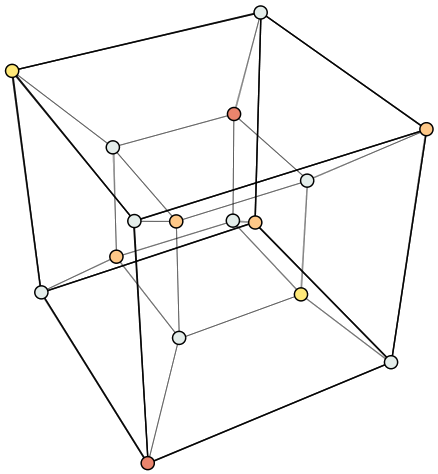
\includegraphics[scale=0.3]{./tesseract_fig1.png}}
	\column{0.5\textwidth}
	\begin{itemize}
		\item Рассматриваемая нами модель имеет координаты $(x_1,x_2,x_3,x_4) \in R^4$, такие, что $x_1 \in [ -1,1 ]$.
		\item Ограгичивается 8 гиперплоскостями	
		\item Имеет 8 трехмерных граней, 24 двумерных, 32 ребра и 16 вершин.
	\end{itemize}
	\clearpage
\end{columns}

%\begin{columns}
%		\column{0.5\textwidth}
% 			Содержимое левого столбца
% 		\column{0.5\textwidth}
% 			Содержимое правого столбца
%\end{columns}
\end{frame}
\begin{frame}
\frametitle{Наглядный процесс формирования отображения тессеракта на трехмерную плоскость}
\begin{center}
\framebox{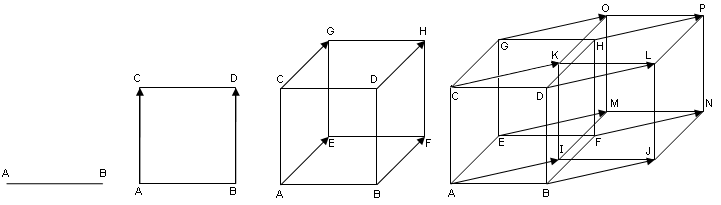
\includegraphics[scale=0.4]{./make_tess.png}}
\end{center}
\\

Наглядный процесс, как точка $A$ переходит постепенно в гиперкуб, приобретая новые размерности
\end{frame}
\begin{frame}
	%THESIS
	Раскрытие тезиса здесь.
\end{frame}
\end{document}
